\documentclass[11pt]{article}
\usepackage[margin=1.1in]{geometry}
\usepackage{amsmath,amssymb}
\usepackage{graphicx}
\usepackage[colorlinks=true,linkcolor=blue,citecolor=blue,urlcolor=blue]{hyperref}
\usepackage{authblk}
\usepackage{tikz}
\usetikzlibrary{positioning,arrows.meta}

\newcommand{\ket}[1]{\left|#1\right\rangle}

\title{\textbf{Temporal-Imaging-Enhanced Dispersive-Optics Quantum Key Distribution: Approaching the Schmidt Limit of Energy--Time Entanglement}}

% =====================================================================
% NOTE TO AUTHOR: replace the placeholder below with your name.
% Per arXiv and APS policy, AI systems may not be listed as authors.
% AI assistance may be noted in the Acknowledgments if you wish.
% =====================================================================
\author[1]{Irfan Ali-Khan}
\affil[1]{Independent Researcher, Saratoga, California, USA}
\date{\today}

\begin{document}
\maketitle

\begin{abstract}
Energy--time entangled photon pairs generated by continuous-wave-pumped spontaneous parametric down-conversion carry a Schmidt number $K = T_{\mathrm{coh}}/\tau_c \sim 10^5$--$10^6$, corresponding to 16--20 bits of potential key per coincidence, yet demonstrated high-dimensional quantum key distribution (QKD) systems extract only 3--7 bits, limited principally by single-photon detector timing jitter. We propose incorporating quantum temporal imaging into entanglement-based time--energy QKD: single-photon time lenses placed inside the trusted receivers magnify the biphoton arrival-time structure before detection, reducing the effective timing resolution below the detector jitter by the temporal magnification $M$. All required components---picosecond-resolution single-photon time lenses with $M>150$, sub-3-ps-jitter superconducting nanowire detectors, and dispersive-optics security checks based on nonlocal dispersion cancellation---have been demonstrated separately; to our knowledge their integration into a QKD protocol, with an accompanying rate and security analysis, has not been considered. We further introduce a nonlocal configuration in which the chromatic dispersion of the transmission fiber itself serves as the input element of a distributed temporal-imaging system completed entirely within one party's laboratory. We analyze the secret-key gain as a function of magnification and lens efficiency, identify a detector-saturation-limited regime in which temporal magnification increases the key rate essentially without loss penalty, and estimate that 13--15 bits per coincidence are within reach of demonstrated hardware, approaching the 17.3-bit correlation-time floor as lens point-spread widths reach the 100-fs scale. Combining demonstrated source, detector, and lens parameters with wavelength-division multiplexing, the protocol projects secret-key rates of order $10^8$ bits per second: roughly two orders of magnitude beyond the highest rates demonstrated with energy--time entangled photons to date, and at parity with the highest secret-key rate yet demonstrated by any QKD system, achieved here in an entanglement-based architecture at an order-of-magnitude higher photon information efficiency. Security follows the dispersive-optics framework, with the time lens entering as a characterized local operation of the trusted receiver, and avoids the postselection loophole of Franson interferometry.
\end{abstract}

\section{Introduction}
\label{sec:intro}

The arrival times of energy--time entangled photon pairs constitute one of the largest naturally occurring alphabets in quantum communication. For pairs produced by continuous-wave (cw) pumped spontaneous parametric down-conversion (SPDC), the two-photon temporal wave function factorizes into a correlation envelope of width $\tau_c \sim 100$~fs, set by the phase-matching or filter bandwidth, and a coherence envelope of width $T_{\mathrm{coh}} \sim 0.1$--$1~\mu$s, set by the inverse pump linewidth. The Schmidt number of this state, $K \simeq T_{\mathrm{coh}}/\tau_c$ \cite{LawEberly2004,AliKhanHowell2006}, counts its information eigenmodes and routinely reaches $10^5$--$10^6$: in principle 16--20 bits of shared randomness per detected pair.

Large-alphabet QKD exploiting this resource was demonstrated in 2007 using binned arrival-time measurements secured by Franson interferometry, achieving 4 bits per coincidence within a 5\% error bound, with an alphabet exceeding 10 bits per pair at higher noise \cite{AliKhan2007}. In the years since, the field has advanced along several fronts reviewed in Sec.~\ref{sec:prior}: dispersive optics has replaced interferometric security checks \cite{Mower2013,Lee2014}, security proofs against collective and coherent attacks have been established \cite{Zhang2014,Niu2016}, layered error-correction codes have raised the photon information efficiency to 6.9 bits per coincidence \cite{Zhong2015}, and superconducting nanowire single-photon detectors (SNSPDs) have reached sub-3-ps jitter \cite{Korzh2020}.

Yet a large gap remains between demonstrated photon information efficiencies and the Schmidt limit, and its dominant cause is unchanged from 2007: \emph{the timing resolution of single-photon detection exceeds the biphoton correlation time by one to three orders of magnitude}. A correlation feature of width 100~fs read out with even a heroic 3-ps detector pair wastes a factor of $\sim 40$ in resolution, or about 5 bits per pair; with practical 30--70-ps detectors the waste approaches 10 bits. Source brightness, channel loss, and reconciliation efficiency have all improved dramatically; the resolution mismatch has not.

This paper proposes closing that gap with quantum temporal imaging. A time lens---a quadratic temporal phase imparted by electro-optic modulation or nonlinear wave mixing, combined with input and output dispersion---realizes the temporal analogue of an optical magnifier \cite{KolnerNazarathy1989,Kolner1994,Salem2013}. Operated on single photons, time lenses have compressed and expanded single-photon bandwidths \cite{Karpinski2017,Donohue2016}, magnified the temporal correlation function of entangled pairs beyond the reach of direct detection \cite{Mittal2017}, and, most relevantly, achieved input-referred timing resolutions of $\sim$1--2~ps with magnification $M = 158$, explicitly sufficient to overcome SNSPD jitter \cite{Joshi2022}. We propose placing such magnifiers inside the trusted receivers of a dispersive-optics QKD (DO-QKD) link, so that the arrival-time alphabet is read out with an effective resolution $\sim \tau_j / M$ rather than $\tau_j$, where $\tau_j$ is the detector jitter. The security architecture of DO-QKD carries over with the lens entering as a characterized local operation, and the protocol inherits immunity to the postselection loophole that afflicts Franson-based security checks \cite{Aerts1999,Jogenfors2015}.

We make four contributions. First, we specify a complete protocol (Sec.~\ref{sec:protocol}) integrating temporal magnification, dispersive-optics security, layered reconciliation, and wavelength-division multiplexing. Second, we derive the photon information efficiency as a function of magnification, lens point-spread width, lens efficiency, and detector jitter, and obtain break-even conditions under which the lens increases the secret-key rate (Sec.~\ref{sec:theory}). Third, we identify the detector-saturation-limited regime---increasingly the relevant regime for bright waveguide sources---in which magnification raises the key rate essentially without loss penalty, because lens insertion loss can be compensated at the source without exceeding the detector count-rate ceiling (Sec.~\ref{sec:rates}). Fourth, we introduce and analyze, at the Gaussian-state level, a \emph{nonlocal} temporal-imaging configuration in which the dispersion of the deployed fiber itself acts as the imaging system's input element, with the lens and output dispersion residing entirely in one laboratory (Sec.~\ref{sec:nonlocal}); the formal tools for this analysis exist in the temporal-entanglement propagation literature \cite{TsangPsaltis2006,Patera2017} but, to our knowledge, this operational use and its security treatment are new.

We have attempted to delineate precisely what is and is not new here, and we encourage the reader to consult Sec.~\ref{sec:prior} before the technical sections.

\section{Relation to prior work}
\label{sec:prior}

Because the present proposal is a synthesis as much as an invention, we state explicitly which ingredients are established.

\emph{Large-alphabet time--energy QKD.} The use of binned arrival times of energy--time entangled pairs as a large alphabet, with conjugate-basis monitoring for security, originates with Ref.~\cite{AliKhan2007}, building on the information-content analysis of Ref.~\cite{AliKhanHowell2006} and Franson interferometry \cite{Franson1989}. Time--energy entanglement is well preserved over long fiber links \cite{Tittel1998,Marcikic2004}, and higher-dimensional encoding confers noise robustness \cite{Cerf2002}.

\emph{Dispersive-optics QKD.} Replacing Franson interferometers with group-velocity dispersion---normal on one side, anomalous on the other---so that frequency correlations are read out as timing correlations via nonlocal dispersion cancellation \cite{Franson1992,Baek2009}, was proposed in Ref.~\cite{Mower2013}. Security against collective attacks via time--frequency covariance-matrix (TFCM) estimation was proven in Ref.~\cite{Zhang2014}, extended to finite-key composable security in Ref.~\cite{Niu2016}, and demonstrated experimentally in Ref.~\cite{Lee2014}. A recent demonstration extends dispersive-optics security to large-alphabet time-bin encoding and EPR steering \cite{Chang2024}. The idea of trading temporal against spectral encoding to match detector capabilities, including dense wavelength-division multiplexing (DWDM) of the SPDC bandwidth, appears in Ref.~\cite{Mower2011}; related hybrid time--frequency schemes are the subject of U.S.~Patent~No.~8,744,086 (2014).

\emph{High photon-information efficiency and reconciliation.} Layered (multilevel) low-density parity-check reconciliation matched to jitter-dominated error statistics achieved 6.9 bits per coincidence \cite{Zhong2015}, with field demonstrations following \cite{Lee2016}. Provably secure time-bin qudit QKD with decoy states reached record rates in Ref.~\cite{Islam2017}. Information-theoretic treatments of jitter-limited secret-key rates and tailored reconciliation codes are given in Ref.~\cite{Boutros2023}.

\emph{Quantum temporal imaging.} Temporal imaging of classical waveforms is a mature field \cite{KolnerNazarathy1989,Kolner1994,Salem2013}. At the quantum level, time lenses have engineered the spectra of entangled photons \cite{Donohue2016}, compressed single-photon bandwidths electro-optically \cite{Karpinski2017}, magnified two-photon temporal correlation functions past the detector-resolution barrier \cite{Mittal2017}, and reached picosecond input-referred resolution at the single-photon level with $M=158$ \cite{Joshi2022}. The propagation of temporal entanglement through dispersive and temporal-imaging systems was analyzed in Refs.~\cite{TsangPsaltis2006,Patera2017}.

\emph{Security loopholes of Franson interferometry.} The postselection inherent in Franson interferometry admits local-realistic models \cite{Aerts1999} and has been exploited in a demonstrated classical-light attack \cite{Jogenfors2015}; dispersive-optics security checks involve no path postselection and are not subject to this attack.

\emph{What is new here.} To the best of our knowledge: (i) the incorporation of single-photon temporal magnification into the key-generation basis of an entanglement-based QKD protocol, with quantitative photon-information-efficiency and break-even analysis, has not been proposed or analyzed; (ii) the observation that, in the detector-saturation-limited regime, temporal magnification raises the secret-key rate essentially free of its insertion-loss penalty is new; (iii) the nonlocal temporal-imaging configuration of Sec.~\ref{sec:nonlocal}, in which deployed-fiber dispersion serves as the input element of a distributed magnifier for the biphoton correlation coordinate, has not been proposed for QKD, and its security discussion is new; and (iv) the system-level synthesis with magnification-aware layered reconciliation is new. We claim no priority on any individual component, and we would be grateful to learn of relevant work we have missed.

\section{Protocol}
\label{sec:protocol}

The protocol operates on energy--time entangled pairs distributed from a central (or Alice-held) source, with one photon delivered to each of Alice and Bob over telecom fiber. The steps are as follows.

\begin{enumerate}
\item \textbf{Distribution.} A cw-pumped waveguide SPDC source (e.g., periodically poled KTP or lithium niobate \cite{Zhong2012}) produces frequency-anticorrelated pairs of correlation time $\tau_c \sim 100$~fs and coherence time $T_{\mathrm{coh}}$ set by the pump linewidth. A shared, public clock defines frames of duration $T_f$.
\item \textbf{Passive basis choice.} Each party directs each incoming photon with a fixed, passive beam splitter to one of two arms. The \emph{time arm} contains a single-photon temporal magnifier (input dispersion, time lens, output dispersion; magnification $M$) followed by an SNSPD and a high-resolution time tagger. The \emph{dispersed arm} applies group-delay dispersion (GDD) $+D$ in Alice's receiver and $-D$ in Bob's, followed by direct SNSPD detection, exactly as in DO-QKD \cite{Mower2013}.
\item \textbf{Measurement.} All detection events are time-tagged relative to the shared clock. Arrival times registered behind the magnifier are divided by $M$ (about the lens's temporal field of view) to refer them to the input time axis.
\item \textbf{Sifting.} Alice and Bob publicly announce, per frame, which arm fired (not the time tag). Time--time coincidences form the raw key; dispersed--dispersed coincidences form the security-check ensemble; mixed-basis events are discarded or used for calibration.
\item \textbf{Parameter estimation.} From the time-basis ensemble the parties estimate the arrival-time correlation variance; from the dispersed-basis ensemble they estimate the dispersed correlation variance, which through nonlocal dispersion cancellation \cite{Franson1992} bounds the frequency-correlation variance. Together these constrain the TFCM, upper-bounding Eve's Holevo information per the security analyses of Refs.~\cite{Zhang2014,Niu2016}. A randomly selected subset of time-arm events, routed around the magnifier by a calibrated bypass switch, audits the magnification and lens calibration.
\item \textbf{Reconciliation and privacy amplification.} Each retained arrival time within its frame is expanded into $b$ bit layers (most-significant first). Layered LDPC codes with per-layer rates matched to the jitter-concentrated error profile reconcile the key without discarding events \cite{Zhong2015,Boutros2023}, and standard privacy amplification compresses by the Holevo bound plus finite-size terms \cite{ShorPreskill2000,Niu2016}.
\end{enumerate}

The architecture is sketched in Fig.~\ref{fig:arch}.

\begin{figure}[t]
\centering
\resizebox{\textwidth}{!}{%
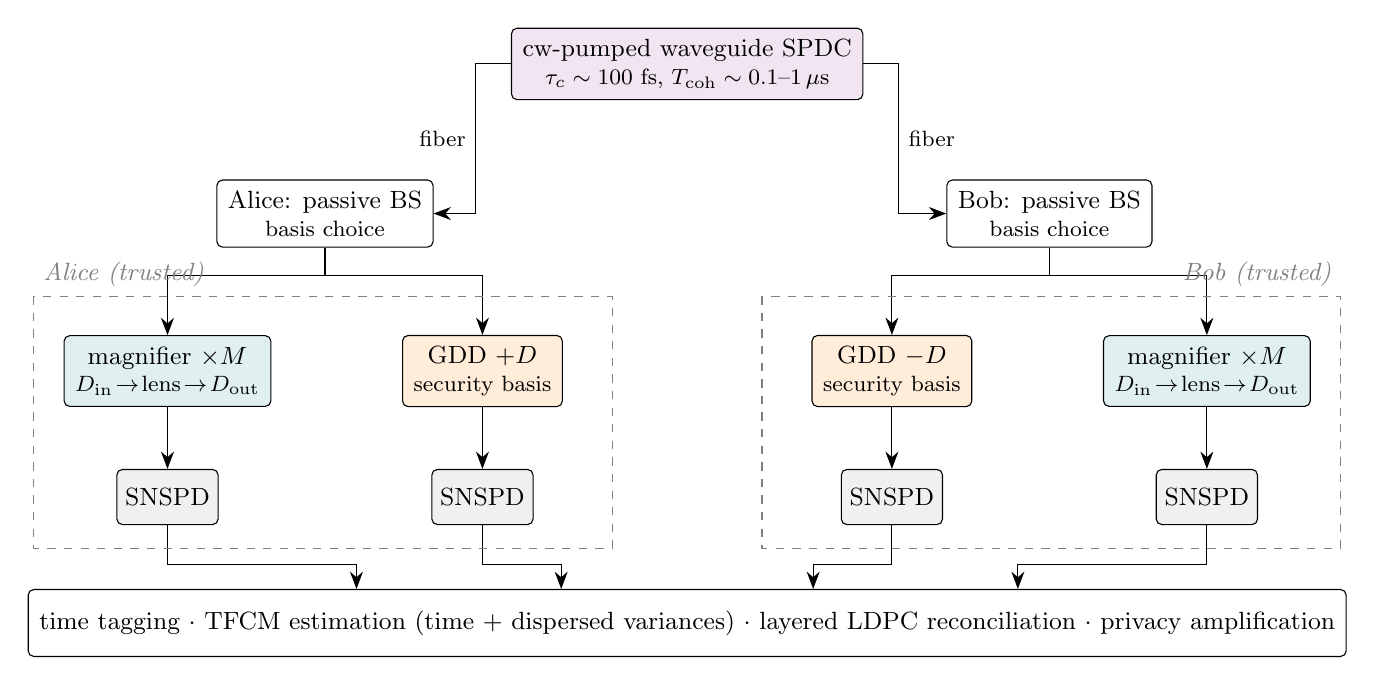
\begin{tikzpicture}[
  >={Stealth[length=2.2mm]},
  box/.style={draw, rounded corners=2pt, align=center, minimum height=8.5mm, inner sep=4pt, font=\small},
  det/.style={draw, rounded corners=2pt, align=center, minimum height=7mm, inner sep=3pt, font=\small, fill=gray!12},
  lab/.style={font=\small\itshape},
  node distance=5mm and 7mm
]
% Source
\node[box, fill=violet!10] (src) at (0,0) {cw-pumped waveguide SPDC\\[-1pt] {\footnotesize $\tau_c\sim 100$ fs, $T_{\mathrm{coh}}\sim 0.1$--$1\,\mu$s}};

% Beam splitters
\node[box] (absplit) at (-4.6,-1.9) {Alice: passive BS\\[-1pt] {\footnotesize basis choice}};
\node[box] (bbsplit) at (4.6,-1.9) {Bob: passive BS\\[-1pt] {\footnotesize basis choice}};

% Alice arms
\node[box, fill=teal!12] (amag) at (-6.6,-3.9) {magnifier $\times M$\\[-1pt] {\footnotesize $D_{\mathrm{in}}\!\to\!\text{lens}\!\to\!D_{\mathrm{out}}$}};
\node[box, fill=orange!15] (adisp) at (-2.6,-3.9) {GDD $+D$\\[-1pt] {\footnotesize security basis}};
\node[det] (adet1) at (-6.6,-5.5) {SNSPD};
\node[det] (adet2) at (-2.6,-5.5) {SNSPD};

% Bob arms
\node[box, fill=orange!15] (bdisp) at (2.6,-3.9) {GDD $-D$\\[-1pt] {\footnotesize security basis}};
\node[box, fill=teal!12] (bmag) at (6.6,-3.9) {magnifier $\times M$\\[-1pt] {\footnotesize $D_{\mathrm{in}}\!\to\!\text{lens}\!\to\!D_{\mathrm{out}}$}};
\node[det] (bdet1) at (2.6,-5.5) {SNSPD};
\node[det] (bdet2) at (6.6,-5.5) {SNSPD};

% Post-processing
\node[box, minimum width=11.6cm] (post) at (0,-7.1) {time tagging $\cdot$ TFCM estimation (time + dispersed variances) $\cdot$ layered LDPC reconciliation $\cdot$ privacy amplification};

% Channel arrows
\draw[->] (src.west) -- ++(-0.45,0) |- node[pos=0.25, left, font=\footnotesize]{fiber} (absplit.east);
\draw[->] (src.east) -- ++(0.45,0) |- node[pos=0.25, right, font=\footnotesize]{fiber} (bbsplit.west);

% Splitter to arms
\draw[->] (absplit.south) -- ++(0,-0.35) -| (amag.north);
\draw[->] (absplit.south) -- ++(0,-0.35) -| (adisp.north);
\draw[->] (bbsplit.south) -- ++(0,-0.35) -| (bdisp.north);
\draw[->] (bbsplit.south) -- ++(0,-0.35) -| (bmag.north);

% Arms to detectors
\draw[->] (amag.south) -- (adet1.north);
\draw[->] (adisp.south) -- (adet2.north);
\draw[->] (bdisp.south) -- (bdet1.north);
\draw[->] (bmag.south) -- (bdet2.north);

% Detectors to post-processing
\draw[->] (adet1.south) -- ++(0,-0.5) -| ([xshift=-4.2cm]post.north);
\draw[->] (adet2.south) -- ++(0,-0.5) -| ([xshift=-1.6cm]post.north);
\draw[->] (bdet1.south) -- ++(0,-0.5) -| ([xshift=1.6cm]post.north);
\draw[->] (bdet2.south) -- ++(0,-0.5) -| ([xshift=4.2cm]post.north);

% Trusted-lab boxes
\draw[dashed, gray] (-8.3,-2.95) rectangle (-0.95,-6.15);
\node[lab, gray, anchor=south west] at (-8.3,-2.95) {Alice (trusted)};
\draw[dashed, gray] (0.95,-2.95) rectangle (8.3,-6.15);
\node[lab, gray, anchor=south east] at (8.3,-2.95) {Bob (trusted)};
\end{tikzpicture}%
}
\caption{Protocol architecture. Each party passively routes incoming photons either to a \emph{time arm}, where a single-photon temporal magnifier ($\times M$) precedes the SNSPD so that arrival times are resolved at $\sim\tau_j/M$, or to a \emph{dispersed arm} carrying group-delay dispersion of opposite sign at the two receivers; nonlocal dispersion cancellation renders the dispersed-basis coincidence width a probe of the frequency correlations, and the two measured variances jointly constrain the time--frequency covariance matrix that bounds Eve's information \cite{Mower2013,Zhang2014}. A calibrated bypass switch (not shown) routes a random subset of time-arm events around the magnifier for calibration auditing. In the nonlocal variant of Sec.~\ref{sec:nonlocal}, Bob's magnifier is removed entirely and the deployed fiber's dispersion serves as $D_{\mathrm{in}}$ of a distributed imaging system completed in Alice's receiver.}
\label{fig:arch}
\end{figure}

The SPDC bandwidth ($\sim$THz) may be demultiplexed into $N_{\mathrm{ch}}$ anticorrelated DWDM channel pairs, each running the protocol in parallel on its own detector pair \cite{Mower2011}; this multiplies throughput and defers detector saturation, and is assumed in the rate estimates of Sec.~\ref{sec:rates}.

\section{Information efficiency with temporal magnification}
\label{sec:theory}

\subsection{State and resolution model}

With a cw pump of frequency $\omega_p$, the post-filter biphoton amplitude is well approximated by
\begin{equation}
\ket{\psi} \propto \int dt_1\, dt_2\; e^{-(t_1-t_2)^2/4\tau_c^2}\; e^{-(t_1+t_2)^2/16T_{\mathrm{coh}}^2}\; e^{-i\omega_p (t_1+t_2)/2}\, \hat a_1^\dagger(t_1)\hat a_2^\dagger(t_2)\ket{0},
\label{eq:state}
\end{equation}
with Schmidt number $K \simeq T_{\mathrm{coh}}/\tau_c$ \cite{LawEberly2004,Grice1997}. The arrival-time difference $t_- = t_1 - t_2$ carries the key correlations; the maximum extractable information per pair is $\log_2 K$.

Detection introduces, per receiver, a Gaussian-equivalent timing error $\epsilon$ combining detector jitter $\tau_j$ and, when a magnifier of magnification $M$ and input-referred point-spread (impulse-response) width $\delta\tau_L$ is present,
\begin{equation}
\epsilon = \sqrt{\left(\tau_j/M\right)^2 + \delta\tau_L^2}\,,
\qquad
\sigma_{\mathrm{obs}} = \sqrt{\tau_c^2 + \epsilon_A^2 + \epsilon_B^2}\,,
\label{eq:resolution}
\end{equation}
where $\sigma_{\mathrm{obs}}$ is the observed width of the coincidence peak in $t_-$. Without magnifiers ($M=1$, $\delta\tau_L=0$), $\sigma_{\mathrm{obs}} \approx \sqrt{2}\,\tau_j$ for $\tau_j \gg \tau_c$. The demonstrated single-photon magnifier of Ref.~\cite{Joshi2022} corresponds to $M=158$ with input-referred resolution $\approx 1.3$--$2$~ps inclusive of electronics; electro-optic lenses \cite{Karpinski2017} trade aperture against point-spread width and are projected to reach sub-picosecond $\delta\tau_L$ with deeper phase modulation.

Binning $t_-$ within the frame at width $\delta = \alpha\, \sigma_{\mathrm{obs}}$ (guard factor $\alpha \approx 3$--5, with residual neighbor-bin errors absorbed by the layered code) yields an alphabet $D = T_f/\delta$ and an ideal photon information efficiency
\begin{equation}
I_{AB} \approx \log_2 \frac{T_f}{\alpha\, \sigma_{\mathrm{obs}}}\,.
\label{eq:pie}
\end{equation}
The gain from magnification is therefore
\begin{equation}
\Delta I = I_{AB}(M) - I_{AB}(1) \approx \log_2 \frac{\sqrt{2}\,\tau_j}{\sqrt{\tau_c^2 + 2\left[(\tau_j/M)^2 + \delta\tau_L^2\right]}}\,.
\label{eq:gain}
\end{equation}
Two regimes follow. With state-of-the-art $\tau_j = 3$~ps SNSPDs \cite{Korzh2020} and $\delta\tau_L = 0.5$~ps, $M \gtrsim 10$ gives $\Delta I \approx 2.4$ bits. With practical $\tau_j = 30$~ps detectors and the demonstrated lens of Ref.~\cite{Joshi2022} ($M=158$, $\delta\tau_L \approx 1.3$~ps), $\Delta I \approx 4.5$ bits---and, notably, the combination of an inexpensive detector and a demonstrated lens outperforms the most exotic detector alone. Magnification substitutes a room-temperature optical component for cryogenic jitter engineering. For the frame parameters used throughout this paper ($T_f = 64$~ns, $\alpha = 4$), the correlation-time floor itself lies at $\log_2[T_f/(\alpha\tau_c)] = 17.3$ bits per coincidence.

\subsection{Break-even against lens loss}
\label{sec:breakeven}

A magnifier has finite efficiency $\eta_L$ (conversion plus insertion; $\eta_L \sim 0.2$--0.5 for four-wave-mixing lenses, with electro-optic lenses potentially higher). In the \emph{source-limited} regime, where the coincidence rate $R_c$ is proportional to delivered pair flux, the secret-key rate scales as $R_c\, \eta_L\, I_{\mathrm{sec}}(M)$ in the time basis, so the lens helps when
\begin{equation}
\eta_L > \frac{I_{\mathrm{sec}}(1)}{I_{\mathrm{sec}}(M)}\,,
\label{eq:breakeven}
\end{equation}
where $I_{\mathrm{sec}}$ is the secret fraction per coincidence after reconciliation and privacy amplification. For the 30-ps-detector example above ($I$ from $\approx 8.6$ to $\approx 13.1$ bits at $T_f = 64$~ns, $\alpha = 4$), break-even requires only $\eta_L \gtrsim 0.66$; for the 3-ps example the requirement is more stringent. Equation~(\ref{eq:breakeven}) is the honest statement of when the lens pays for itself photon-for-photon.

The more favorable and, for modern systems, more relevant case is the \emph{detector-saturation-limited} regime. Waveguide SPDC sources deliver pair rates far exceeding the maximum useful count rate $R_{\det}^{\max}$ of an SNSPD channel (dead-time and pile-up limited, typically $10^6$--$10^7\,\mathrm{s}^{-1}$). When the operating point is set by $R_{\det}^{\max}$ rather than by available pairs, lens loss is compensated upstream by pump power at no cost to the detected rate, and the key rate becomes
\begin{equation}
R_{\mathrm{key}} \approx N_{\mathrm{ch}}\; R_{\det}^{\max}\, \kappa \; I_{\mathrm{sec}}(M)\,,
\label{eq:satrate}
\end{equation}
with $\kappa$ the coincidence-to-singles ratio: every bit of $\Delta I$ multiplies the key rate directly. The cost reappears only through the multi-pair emission probability per frame, which grows with pump power and feeds the accidental-coincidence floor and Eve's multi-pair information; this is bounded by frame-occupancy statistics in the standard way \cite{Zhang2014,Zhong2015} and constrains the usable $T_f$ and pump strength jointly. We emphasize that Eq.~(\ref{eq:satrate}) is the operating point that bright modern sources actually reach, and it is the regime in which temporal magnification is most valuable.

\subsection{Security considerations}
\label{sec:security}

The security architecture is that of DO-QKD \cite{Mower2013,Zhang2014,Niu2016}: Alice and Bob's measured time-basis and dispersed-basis correlation variances constrain the time--frequency covariance matrix of the joint state delivered by the (adversarial) channel, and Gaussian extremality yields an upper bound on Eve's Holevo information; finite-key corrections follow Ref.~\cite{Niu2016}. Three points specific to the present proposal deserve statement.

First, the magnifier is a \emph{local operation of the trusted receiver}, applied after the channel and after basis selection. As such it cannot increase Eve's information; its calibrated map ($t \to Mt$ within the field of view, efficiency $\eta_L$, point spread $\delta\tau_L$) is inverted in software, and miscalibration appears as excess noise in the estimated time-basis variance, which the security bound treats conservatively (i.e., attributes to Eve). The random lens-bypass audit of Sec.~\ref{sec:protocol} bounds calibration drift and tampering of the lens pump.

Second, the lens's own optical pump (for four-wave-mixing implementations) is a potential side channel: pump leakage correlates with lens timing, and an active Eve might attempt to probe or inject light at lens wavelengths. Standard countermeasures---spectral isolation, watchdog photodiodes, and optical isolators at the receiver input---apply, and the conservative variance accounting above covers residual effects. We flag a full device-level analysis as necessary future work; the situation is analogous to, and no worse than, detector-side channels in any QKD receiver.

Third, because neither basis involves interferometric path postselection, the protocol is structurally immune to the Franson postselection attack \cite{Aerts1999,Jogenfors2015}. Frame postselection (discarding frames without coincident detections) is loss postselection of the kind already treated in the DO-QKD security analyses \cite{Zhang2014,Niu2016}.

\section{Nonlocal temporal magnification}
\label{sec:nonlocal}

We now describe the configuration that we regard as the most physically interesting contribution of this paper. In a frequency-anticorrelated biphoton, group-delay dispersion applied to one photon acts, at the level of the two-photon amplitude in the difference coordinate $t_-$, equivalently to dispersion applied to its partner: writing $\omega_{1,2} = \omega_p/2 \pm \Omega$ for a narrow pump, GDD phases $\exp[i D_A \Omega^2/2]$ and $\exp[i D_B \Omega^2/2]$ applied separately to the two photons combine into a single phase $\exp[i (D_A + D_B)\Omega^2/2]$ on the joint amplitude. This is the content of nonlocal dispersion cancellation \cite{Franson1992,Baek2009,MacLean2018}: only the \emph{sum} of the dispersions broadens the coincidence peak.

Temporal imaging of a waveform requires input dispersion $D_{\mathrm{in}}$, a quadratic phase (focal GDD $D_f$), and output dispersion $D_{\mathrm{out}}$ satisfying the imaging condition
\begin{equation}
\frac{1}{D_{\mathrm{in}}} + \frac{1}{D_{\mathrm{out}}} = \frac{1}{D_f}\,, \qquad M = -\frac{D_{\mathrm{out}}}{D_{\mathrm{in}}}\,,
\label{eq:imaging}
\end{equation}
in direct analogy to the thin-lens equation \cite{KolnerNazarathy1989,Kolner1994}. The observation above implies that, for the biphoton difference coordinate, the three elements of Eq.~(\ref{eq:imaging}) need not reside on the same photon's path. In particular, the uncompensated chromatic dispersion $D_{\mathrm{fib}}$ of Bob's deployed fiber---ordinarily an impairment requiring compensation---can serve as $D_{\mathrm{in}}$, with the time lens and the output dispersion $D_{\mathrm{out}}$ located entirely in Alice's receiver acting on her photon. At the Gaussian level, propagating the state of Eq.~(\ref{eq:state}) through this distributed system (the formalism of Refs.~\cite{TsangPsaltis2006,Patera2017} applies directly) is expected to yield a coincidence distribution in $t_-$ magnified by $M$, even though no single photon traverses a complete imaging system, and even though Bob's receiver contains nothing but a detector. We state plainly that this derivation has not been carried through in full here: it is published as an explicitly open claim, labeled as such in the claim ledger accompanying this work, and its confirmation or refutation is invited as a community contribution to the public record of this paper.

Operationally this has three attractive features. (i) Bob's receiver is reduced to a passive splitter, a dispersive element for the security basis, and detectors---all magnification hardware concentrates at Alice, which suits asymmetric deployments (a central exchange serving thin clients). (ii) The channel's own dispersion is conscripted as a functional element rather than compensated, in the same spirit in which DO-QKD conscripts dispersion for security. (iii) Singles distributions on both sides remain nanosecond-scale featureless blurs; the magnified structure exists only in coincidences, which is operationally pleasant (an intercepting Eve gains nothing detector-resolution-limited to exploit) though we emphasize it confers no security beyond the TFCM bound.

Two honest caveats accompany this proposal. First, the temporal field of view of the lens must cover the arrival-time uncertainty of the photon within a frame; with a cw pump this uncertainty is the full frame, which strains electro-optic apertures. A pulsed or phase-modulated pump that pre-localizes pair generation into known sub-frame slots (at some cost in $T_{\mathrm{coh}}$ and hence $K$), or a triggered lens architecture, addresses this; the optimization of frame structure against lens aperture is an open design problem, for which temporal self-imaging (Talbot) pump combs are a natural candidate. Second, because the lens now acts on a photon that has not traversed the channel, the calibration audit of Sec.~\ref{sec:protocol} must additionally verify the \emph{sign and magnitude} of the deployed-fiber dispersion serving as $D_{\mathrm{in}}$; an Eve with access to the fiber could alter its dispersion, which would appear as a magnification miscalibration. The conservative variance accounting of Sec.~\ref{sec:security} again covers this---altered dispersion inflates the measured time-basis variance and reduces the certified key rather than compromising it---but a dedicated analysis is warranted and is identified as future work.

\section{Rate estimates}
\label{sec:rates}

Table~\ref{tab:rates} assembles representative operating points. We stress that the entries for the proposed protocol are design estimates from Eqs.~(\ref{eq:resolution})--(\ref{eq:satrate}) using demonstrated component parameters, not measurements, and that finite-key, reconciliation-inefficiency ($\beta \approx 0.9$), and privacy-amplification deductions are folded into an assumed secret fraction $I_{\mathrm{sec}} \approx 0.6\, I_{AB}$, consistent with the accounting achieved in Ref.~\cite{Zhong2015}.

\begin{table}[t]
\centering
\begin{tabular}{lllll}
\hline\hline
System & Detector & PIE (bits/coin) & Coincidence rate & Key rate \\
\hline
Ref.~\cite{AliKhan2007} (2007) & SPCM, 350 ps & 4 & $\sim 50$ Hz & $\sim 2\times10^2$ b/s \\
Ref.~\cite{Zhong2015} (2015) & SNSPD, $\sim$70 ps & 6.9 & $\sim 10^6$ s$^{-1}$ & $2.7\times10^6$ b/s \\
Proposed, local lenses & SNSPD, 30 ps; $M{=}158$ & 13 & $10^7$ s$^{-1}$ ($\times N_{\mathrm{ch}}$) & $\sim 10^8$ b/s \\
Proposed, 3 ps + lens & SNSPD, 3 ps; $M{=}30$ & 14--15 & $10^7$ s$^{-1}$ ($\times N_{\mathrm{ch}}$) & $\gtrsim 10^8$ b/s \\
\hline\hline
\end{tabular}
\caption{Representative operating points. PIE: photon information efficiency before secret-fraction deductions; proposed-system rows assume $T_f = 64$~ns, $\alpha = 4$, $\delta\tau_L = 1.3$~ps ($M{=}158$ row, per Ref.~\cite{Joshi2022}) or $0.5$~ps (projected electro-optic lens), DWDM parallelization $N_{\mathrm{ch}} = 8$--16 \cite{Mower2011}, and detector-saturation-limited operation, Eq.~(\ref{eq:satrate}). Channel loss shortens all rates equally and is omitted for comparability.}
\label{tab:rates}
\end{table}

Three observations. First, against the 2007 baseline the proposed system gains roughly six orders of magnitude in key rate, of which approximately three are generational (source brightness, detector efficiency, multiplexing), one to two come from reclaiming alphabet depth via magnification and zero-discard layered reconciliation, and the remainder from saturation-limited operation. Second, against the state of the art \cite{Zhong2015,Islam2017} the distinctive gain of this proposal is the 7--10 bit-per-coincidence increase in PIE at fixed detector technology, worth a factor of $\sim$30--100 in rate when detectors, not photons, are the scarce resource. Third, the protocol degrades gracefully: every parameter ($M$, $T_f$, $\alpha$, layer rates) is computational or locally physical, so the operating point can be re-optimized in post-processing as channel conditions or adversarial activity (reflected in the TFCM estimates) evolve---preserving the software-reoptimization philosophy of Ref.~\cite{AliKhan2007}.

It is fair to ask how the projected $\sim 10^8$~b/s compares with the best QKD systems of any architecture, and whether the exercise is therefore worthwhile. The highest secret-key rate demonstrated to date is 115.8~Mb/s over 10~km of standard fiber, achieved with decoy-state BB84, a multipixel SNSPD, and 2.5-GHz-class clocking \cite{Li2023}; a contemporaneous time-bin system reached 64~Mb/s at 10~km \cite{Grunenfelder2023}, and continuous-variable systems have recently reported still higher composable rates at metropolitan distances in preprint form (e.g., arXiv:2503.14843). Our projection is thus at \emph{parity} with the demonstrated record, not beyond it, and we do not claim raw-rate supremacy over mature prepare-and-measure systems at metro distances. The case for the present protocol is threefold. First, it is entanglement-based: security does not rest on trusting the source, and the architecture extends naturally to untrusted-node and multiuser network settings where prepare-and-measure does not. Second, and centrally, it achieves its rate at a photon information efficiency of order 10 bits per detected coincidence, versus $\lesssim 1$ bit per detected photon for the record systems above; wherever detected photons rather than clock cycles are the scarce resource---long-haul and satellite links, loss-dominated channels, detector-saturation-limited receivers, and heavily multiplexed networks---photon information efficiency, not source clock rate, sets the achievable key rate, and there the advantage of this approach is a genuine order of magnitude. Third, against its own family---entanglement-based time--energy QKD, whose demonstrated rates stand at 2.7~Mb/s in the laboratory \cite{Zhong2015} and 1.2~Mb/s over deployed fiber \cite{Lee2016}---the projected gain is roughly two orders of magnitude.

\section{Discussion}
\label{sec:discussion}

The proposal advanced here is conservative in its physics---every element has been demonstrated---and aggressive only in its integration. The experimental program it implies is staged and each stage is independently publishable: (1) a tabletop demonstration that a single-photon magnifier on one arm of a cw-pumped DO-QKD link increases measured PIE per Eq.~(\ref{eq:gain}); (2) closure of the security loop with TFCM estimation and the lens-bypass audit; (3) the nonlocal configuration over a fiber spool serving as $D_{\mathrm{in}}$; (4) DWDM parallelization. Stage (1) requires only the marriage of two published experimental capabilities \cite{Lee2014,Joshi2022}.

Several theoretical problems remain open and are stated here as invitations. A full multimode (beyond-Gaussian) security analysis incorporating the lens map, its pump side channel, and the nonlocal configuration's dependence on channel dispersion is the most important. The joint optimization of pump format (cw, pulsed, or Talbot-comb), frame structure, and lens aperture is the most practical. And the information-theoretic question of optimal reconciliation when the error kernel is a known, magnification-rescaled jitter distribution connects directly to the coding-theory program of Ref.~\cite{Boutros2023}.

Energy--time entanglement has always promised more bits than our detectors could read. Dispersive optics taught us to let the channel's dispersion stand guard; temporal imaging now offers to let optics, rather than cryogenics, supply the missing resolution. The Schmidt limit is not yet in hand, but for the first time the gap between it and demonstrated hardware is an engineering integration problem rather than a detector-physics problem.

\section*{Note added (12 June 2026)}
Hours after the v1.0.0 release, an author reality check sharpened red-team Finding 3, and per the living-record doctrine of this publication the amendment is absorbed here rather than exiled to errata. Temporal magnification dilates the lens's accepted input window by $M$: an aperture of duration $T_a$ occupies $M T_a$ at the output, so apertures cannot be packed and each lens-plus-detector channel accepts only $\sim 1/M$ of continuous input time under cw pumping. At any useful $M$, this per-channel acceptance penalty overwhelms the $\sim 1.5\times$ gain in bits per detected pair, and the rate projections of Table~\ref{tab:rates} therefore implicitly assume an aperture architecture this paper did not specify. The photon-information-efficiency claims (bits per detected coincidence) are unaffected. The rate projections are now labeled \emph{architecture-dependent}, pending a quantified treatment of one of three candidate architectures: (a) a pulsed or temporal-Talbot pump aligning pair generation into accepted apertures (repetition rate $\lesssim 1/(M T_a)$, with a correspondingly reduced frame alphabet); (b) $M$-way time-demultiplexing of the magnified output onto a detector array; or (c) wavelength-division parallelization scaled toward $\sim M$ channels. Claim C07 in the public ledger is amended accordingly, and the full statement is recorded as issue~\#1 of the public repository. The archived v1.0.0 of record remains frozen at Zenodo; this note is part of the living record that supersedes it.

\section*{Reproducibility}
Every quantitative claim in this paper (Schmidt numbers, magnification gains, break-even efficiencies, Table~\ref{tab:rates}, and rate comparisons) is recomputed from its stated assumptions by an open verification script, \texttt{verify\_numbers.py}, distributed with this manuscript. Readers are invited to rerun it, vary the assumptions, and report discrepancies.

\section*{Acknowledgments}
% NOTE TO AUTHOR: edit as you see fit. arXiv policy permits (and increasingly
% expects) disclosure of substantive AI assistance; AI systems may not be authors.
The author acknowledges the substantive use of an AI assistant (Claude, Anthropic) in this work, including literature search, prior-art analysis, drafting, rate modeling, and the figure and verification tooling. Beyond its scientific content, this paper is offered as a demonstration of AI-assisted independent research published in a verified-open format, whose governing invariant is honest labeling rather than universal verification: every claim is typed and routed to a verifier in a public claim ledger; numerical claims are recomputed by an open script under continuous integration; citations are audited against primary sources; and claims that no human or machine has independently verified---including the nonlocal-imaging derivation of Sec.~\ref{sec:nonlocal}---are labeled as open rather than asserted. The author's review was conducted at the level of consistency, plausibility, and reality checks on end results, not independent re-derivation, and responsibility for the work rests with the author on that explicitly stated basis. Confirmations, refutations, and corrections are invited through the public repository accompanying this paper, where they become part of its versioned record.

\begin{thebibliography}{99}

\bibitem{AliKhan2007} I. Ali-Khan, C. J. Broadbent, and J. C. Howell, Large-alphabet quantum key distribution using energy-time entangled bipartite states, Phys. Rev. Lett. \textbf{98}, 060503 (2007).

\bibitem{AliKhanHowell2006} I. Ali Khan and J. C. Howell, Experimental demonstration of high two-photon time-energy entanglement, Phys. Rev. A \textbf{73}, 031801(R) (2006).

\bibitem{Franson1989} J. D. Franson, Bell inequality for position and time, Phys. Rev. Lett. \textbf{62}, 2205 (1989).

\bibitem{Franson1992} J. D. Franson, Nonlocal cancellation of dispersion, Phys. Rev. A \textbf{45}, 3126 (1992).

\bibitem{Mower2013} J. Mower, Z. Zhang, P. Desjardins, C. Lee, J. H. Shapiro, and D. Englund, High-dimensional quantum key distribution using dispersive optics, Phys. Rev. A \textbf{87}, 062322 (2013).

\bibitem{Zhang2014} Z. Zhang, J. Mower, D. Englund, F. N. C. Wong, and J. H. Shapiro, Unconditional security of time-energy entanglement quantum key distribution using dual-basis interferometry, Phys. Rev. Lett. \textbf{112}, 120506 (2014).

\bibitem{Niu2016} M. Y. Niu, F. Xu, J. H. Shapiro, and F. Furrer, Finite-key analysis for time-energy high-dimensional quantum key distribution, Phys. Rev. A \textbf{94}, 052323 (2016).

\bibitem{Lee2014} C. Lee, Z. Zhang, G. R. Steinbrecher, H. Zhou, J. Mower, T. Zhong, L. Wang, X. Hu, R. D. Horansky, V. B. Verma, A. E. Lita, R. P. Mirin, F. Marsili, M. D. Shaw, S. W. Nam, G. W. Wornell, F. N. C. Wong, J. H. Shapiro, and D. Englund, Entanglement-based quantum communication secured by nonlocal dispersion cancellation, Phys. Rev. A \textbf{90}, 062331 (2014).

\bibitem{Zhong2015} T. Zhong, H. Zhou, R. D. Horansky, C. Lee, V. B. Verma, A. E. Lita, A. Restelli, J. C. Bienfang, R. P. Mirin, T. Gerrits, S. W. Nam, F. Marsili, M. D. Shaw, Z. Zhang, L. Wang, D. Englund, G. W. Wornell, J. H. Shapiro, and F. N. C. Wong, Photon-efficient quantum key distribution using time-energy entanglement with high-dimensional encoding, New J. Phys. \textbf{17}, 022002 (2015).

\bibitem{Lee2016} C. Lee, D. Bunandar, Z. Zhang, G. R. Steinbrecher, P. B. Dixon, F. N. C. Wong, J. H. Shapiro, S. A. Hamilton, and D. Englund, High-rate field demonstration of large-alphabet quantum key distribution, arXiv:1611.01139 (2016).

\bibitem{Islam2017} N. T. Islam, C. C. W. Lim, C. Cahall, J. Kim, and D. J. Gauthier, Provably secure and high-rate quantum key distribution with time-bin qudits, Sci. Adv. \textbf{3}, e1701491 (2017).

\bibitem{Mower2011} J. Mower, F. N. C. Wong, J. H. Shapiro, and D. Englund, Dense wavelength division multiplexed quantum key distribution using entangled photons, arXiv:1110.4867 (2011).

\bibitem{Jogenfors2015} J. Jogenfors, A. M. Elhassan, J. Ahrens, M. Bourennane, and J.-\AA. Larsson, Hacking the Bell test using classical light in energy-time entanglement-based quantum key distribution, Sci. Adv. \textbf{1}, e1500793 (2015).

\bibitem{Aerts1999} S. Aerts, P. Kwiat, J.-\AA. Larsson, and M. \.Zukowski, Two-photon Franson-type experiments and local realism, Phys. Rev. Lett. \textbf{83}, 2872 (1999).

\bibitem{KolnerNazarathy1989} B. H. Kolner and M. Nazarathy, Temporal imaging with a time lens, Opt. Lett. \textbf{14}, 630 (1989).

\bibitem{Kolner1994} B. H. Kolner, Space-time duality and the theory of temporal imaging, IEEE J. Quantum Electron. \textbf{30}, 1951 (1994).

\bibitem{Salem2013} R. Salem, M. A. Foster, and A. L. Gaeta, Application of space-time duality to ultrahigh-speed optical signal processing, Adv. Opt. Photon. \textbf{5}, 274 (2013).

\bibitem{Karpinski2017} M. Karpi\'nski, M. Jachura, L. J. Wright, and B. J. Smith, Bandwidth manipulation of quantum light by an electro-optic time lens, Nat. Photonics \textbf{11}, 53 (2017).

\bibitem{Donohue2016} J. M. Donohue, M. Mastrovich, and K. J. Resch, Spectrally engineering photonic entanglement with a time lens, Phys. Rev. Lett. \textbf{117}, 243602 (2016).

\bibitem{Mittal2017} S. Mittal, V. V. Orre, A. Restelli, R. Salem, E. A. Goldschmidt, and M. Hafezi, Temporal and spectral manipulations of correlated photons using a time lens, Phys. Rev. A \textbf{96}, 043807 (2017).

\bibitem{Joshi2022} C. Joshi, B. M. Sparkes, A. Farsi, T. Gerrits, V. Verma, S. Ramelow, S. W. Nam, and A. L. Gaeta, Picosecond-resolution single-photon time lens for temporal mode quantum processing, Optica \textbf{9}, 364 (2022).

\bibitem{TsangPsaltis2006} M. Tsang and D. Psaltis, Propagation of temporal entanglement, Phys. Rev. A \textbf{73}, 013822 (2006).

\bibitem{Patera2017} G. Patera, J. Shi, D. B. Horoshko, and M. I. Kolobov, Quantum temporal imaging: application of a time lens to quantum optics, J. Opt. \textbf{19}, 054001 (2017).

\bibitem{Baek2009} S.-Y. Baek, Y.-W. Cho, and Y.-H. Kim, Nonlocal dispersion cancellation using entangled photons, Opt. Express \textbf{17}, 19241 (2009).

\bibitem{MacLean2018} J.-P. W. MacLean, J. M. Donohue, and K. J. Resch, Direct characterization of ultrafast energy-time entangled photon pairs, Phys. Rev. Lett. \textbf{120}, 053601 (2018).

\bibitem{Korzh2020} B. Korzh, Q.-Y. Zhao, J. P. Allmaras, S. Frasca, T. M. Autry, E. A. Bersin, A. D. Beyer, R. M. Briggs, B. Bumble, M. Colangelo, et al., Demonstration of sub-3 ps temporal resolution with a superconducting nanowire single-photon detector, Nat. Photonics \textbf{14}, 250 (2020).

\bibitem{Chang2024} K.-C. Chang, M. C. Sarihan, X. Cheng, Z. Zhang, and C. W. Wong, Large-alphabet time-bin quantum key distribution and Einstein-Podolsky-Rosen steering via dispersive optics, Quantum Sci. Technol. \textbf{9}, 015018 (2024).

\bibitem{Boutros2023} J. J. Boutros and E. Soljanin, Time-entanglement QKD: secret key rates and information reconciliation coding, IEEE Trans. Commun. \textbf{71}, 7174 (2023).

\bibitem{LawEberly2004} C. K. Law and J. H. Eberly, Analysis and interpretation of high transverse entanglement in optical parametric down conversion, Phys. Rev. Lett. \textbf{92}, 127903 (2004).

\bibitem{Grice1997} W. P. Grice and I. A. Walmsley, Spectral information and distinguishability in type-II down-conversion with a broadband pump, Phys. Rev. A \textbf{56}, 1627 (1997).

\bibitem{Zhong2012} T. Zhong, F. N. C. Wong, A. Restelli, and J. C. Bienfang, Efficient single-spatial-mode periodically-poled KTiOPO$_4$ waveguide source for high-dimensional entanglement-based quantum key distribution, Opt. Express \textbf{20}, 26868 (2012).

\bibitem{Tittel1998} W. Tittel, J. Brendel, H. Zbinden, and N. Gisin, Violation of Bell inequalities by photons more than 10 km apart, Phys. Rev. Lett. \textbf{81}, 3563 (1998).

\bibitem{Marcikic2004} I. Marcikic, H. de Riedmatten, W. Tittel, H. Zbinden, M. Legr\'e, and N. Gisin, Distribution of time-bin entangled qubits over 50 km of optical fiber, Phys. Rev. Lett. \textbf{93}, 180502 (2004).

\bibitem{Cerf2002} N. J. Cerf, M. Bourennane, A. Karlsson, and N. Gisin, Security of quantum key distribution using d-level systems, Phys. Rev. Lett. \textbf{88}, 127902 (2002).

\bibitem{Li2023} W. Li, L. Zhang, H. Tan, Y. Lu, S.-K. Liao, J. Huang, H. Li, Z. Wang, H.-K. Mao, B. Yan, Q. Li, Y. Liu, Q. Zhang, C.-Z. Peng, L. You, F. Xu, and J.-W. Pan, High-rate quantum key distribution exceeding 110 Mb\,s$^{-1}$, Nat. Photonics \textbf{17}, 416 (2023).

\bibitem{Grunenfelder2023} F. Gr\"unenfelder, A. Boaron, G. V. Resta, M. Perrenoud, D. Rusca, C. Barreiro, R. Houlmann, R. Sax, L. Stasi, S. El-Khoury, E. H\"anggi, N. Bosshard, F. Bussi\`eres, and H. Zbinden, Fast single-photon detectors and real-time key distillation enable high secret-key-rate quantum key distribution systems, Nat. Photonics \textbf{17}, 422 (2023).

\bibitem{ShorPreskill2000} P. W. Shor and J. Preskill, Simple proof of security of the BB84 quantum key distribution protocol, Phys. Rev. Lett. \textbf{85}, 441 (2000).

\end{thebibliography}

\end{document}
